 \section{Cinemática Inversa}


	\subsection{Robot 6}
	   \begin{figure}[H]
	   	\centering
	   	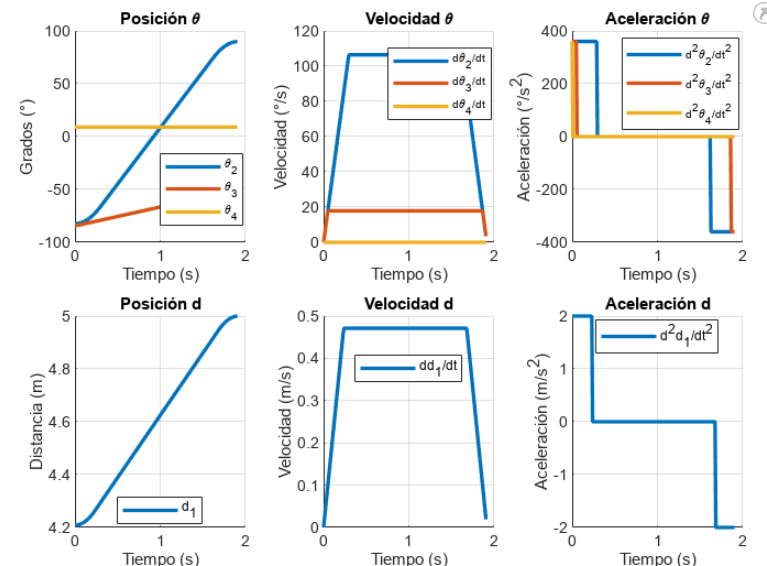
\includegraphics[width=0.8\textwidth]{R6_cinematica_articular}
	   	\caption{Cinemática articular del robot 6: posición, velocidad y aceleración de las articulaciones en función del tiempo.}
	   	\label{fig:cinematica_articular}
	   \end{figure}
	   
	   \begin{figure}[H]
	   	\centering
	   	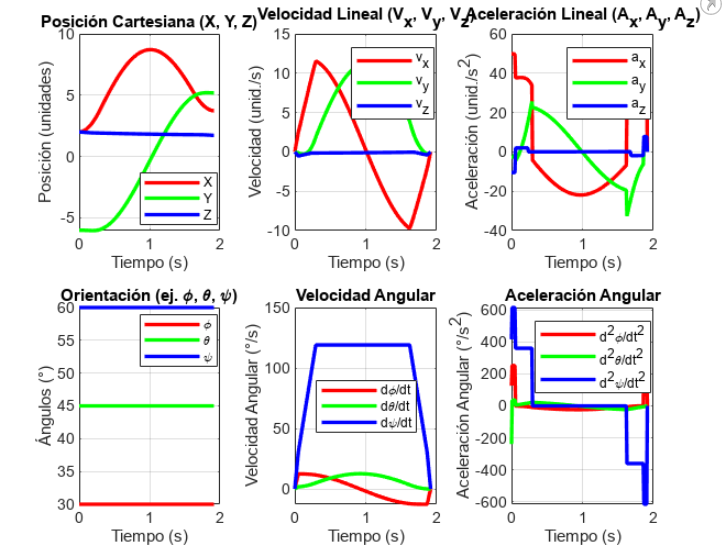
\includegraphics[width=0.8\textwidth]{R6_graficas_1}
	   	\caption{Cinemática cartesiana del robot 6: posición, velocidad y aceleración lineal y angular en función del tiempo.}
	   	\label{fig:cinematica_cartesiana}
	   \end{figure}
	   
	   \begin{figure}[H]
	   	\centering
	   	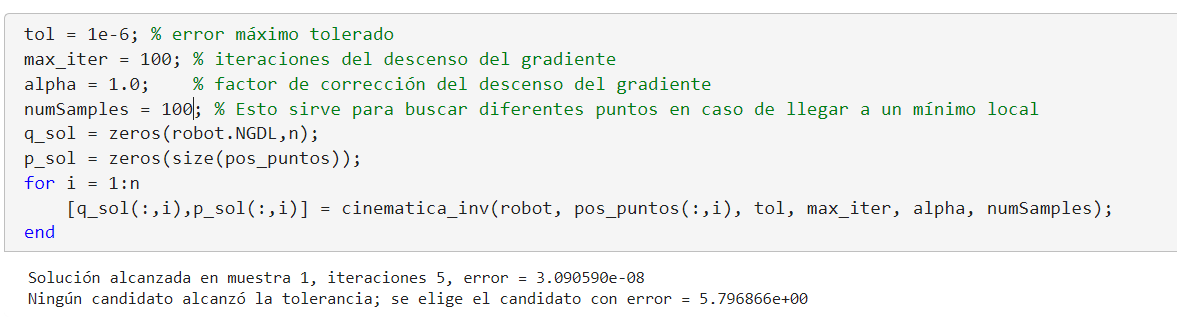
\includegraphics[width=1\textwidth]{R6_error}
	   	\caption{Error del objetivo del robot 6.}
	   	\label{fig:error_objetivo6}
	   \end{figure}
	   
			
			
	\subsection{Robot 7}
	\begin{figure}[H]
		\centering
		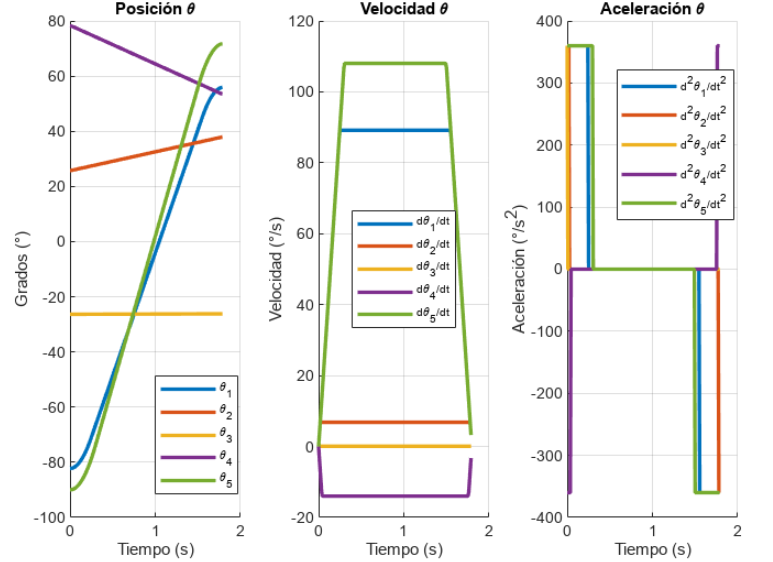
\includegraphics[width=0.65\textwidth]{R7_cinematica_art}
		\caption{Cinemática articular del robot 7: posición, velocidad y aceleración de las articulaciones en función del tiempo.}
		\label{fig:R7_cinematica_articular}
	\end{figure}
	
	\begin{figure}[H]
		\centering
		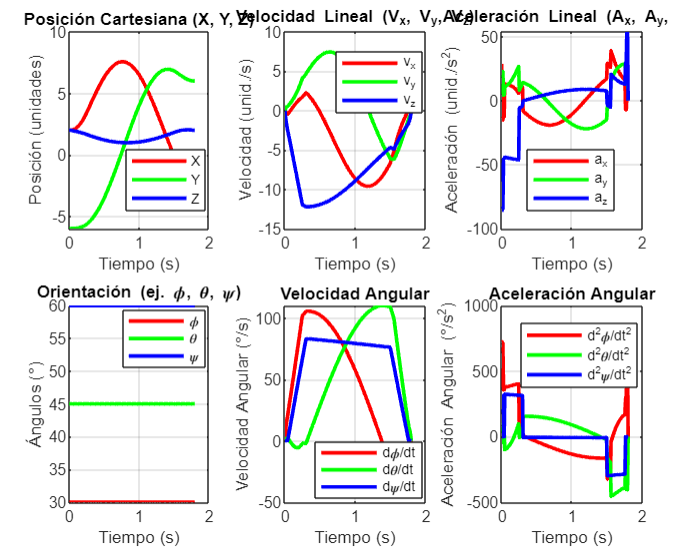
\includegraphics[width=0.65\textwidth]{R7_graficas}
		\caption{Cinemática cartesiana del robot R7: posición, velocidad y aceleración lineal y angular en función del tiempo.}
		\label{fig:R7_cinematica_cartesiana}
	\end{figure}
	
	\begin{figure}[H]
		\centering
		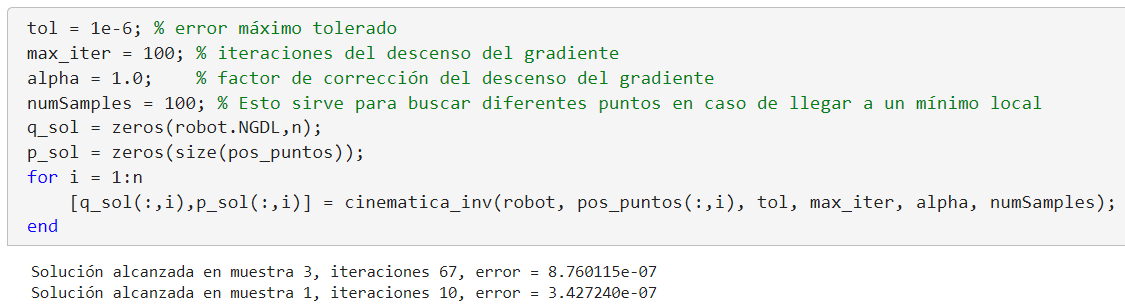
\includegraphics[width=1\textwidth]{R7_error}
		\caption{Error del objetivo del robot 7.}
		\label{fig:R7_error_objetivo7}
	\end{figure}
	
	
